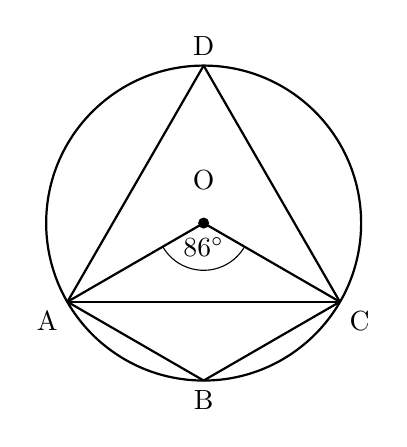
\begin{tikzpicture}

    % Define the center and radius of the circle
    \coordinate (O) at (0, 0.5);     % Center point O
    \def\radius{2}
    
    % Define the points on the circle
    % D at top, A at bottom-left, B at bottom-center, C at bottom-right
    \coordinate (D) at (0, 2.5);                    % Top point
    \coordinate (A) at (-1.73, -0.5);               % Bottom-left point
    \coordinate (B) at (0, -1.5);                   % Bottom point
    \coordinate (C) at (1.73, -0.5);                % Bottom-right point
    
    % Draw the circle
    \draw[thick] (O) circle (\radius);
    
    % Draw the quadrilateral ADBC inscribed in circle
    \draw[thick] (A) -- (D);         % Side AD
    \draw[thick] (D) -- (C);         % Side DC
    \draw[thick] (C) -- (B);         % Side CB
    \draw[thick] (B) -- (A);         % Side BA
    \draw[thick] (A) -- (C);         % Diagonal AC
    
    % Draw lines from O to A and O to C (forming the central angle)
    \draw[thick] (O) -- (A);         % Line OA
    \draw[thick] (O) -- (C);         % Line OC
    
    % Draw the center point O as a filled circle
    \fill (O) circle (2pt);
    
    % Draw the arc for the central angle AOC (86 degrees)
    \draw (O) ++(210:0.6) arc (210:330:0.6);
    
    % Label point D
    \node[above] at (D) {D};
    
    % Label point A
    \node[below left] at (A) {A};
    
    % Label point B
    \node[below] at (B) {B};
    
    % Label point C
    \node[below right] at (C) {C};
    
    % Label point O
    \node[above] at (0, 0.8) {O};
    
    % Label the angle 86 degrees
    \node at (0, 0.2) {$86^{\circ}$};
    
    \end{tikzpicture}